\documentclass[a4paper,10pt]{article}
\usepackage{amsmath,amssymb}
\usepackage{verbatim}
\usepackage{setspace}
\usepackage{color}
\usepackage{tikz}
\usetikzlibrary{shapes,arrows,snakes}

\textheight 700 pt
\textwidth 450 pt
\oddsidemargin 0 pt
\evensidemargin 0 pt
\topmargin -27 pt
\headheight 0 pt
\headsep 0 pt
\parindent 0 pt
\pagestyle{empty}

%% Mathoperators
\DeclareMathOperator{\dive}{div}
\DeclareMathOperator{\grad}{grad}
\DeclareMathOperator{\spann}{span}
\DeclareMathOperator{\nulli}{null}
\DeclareMathOperator{\ind}{ind}
\DeclareMathOperator{\rank}{rank}
\DeclareMathOperator{\kernel}{kernel}
\DeclareMathOperator{\const}{const.}
\DeclareMathOperator{\trace}{tr}
\DeclareMathOperator{\image}{im}
\DeclareMathOperator{\re}{Re}



%%environments
\newcommand{\beq}[1]{\begin{equation}\label{#1}}% equation with labeling
\newcommand{\eeq}{\end{equation}} 

\providecommand{\besu}{\begin{subequations}}
\providecommand{\esu}{\end{subequations}}

%% mathsymbols
\providecommand{\abs}[1]{\lvert#1\rvert}
\providecommand{\abso}[1]{\lvert#1\rvert_1}
\providecommand{\norm}[1]{\lVert#1 \rVert}
\providecommand{\dupa}[2]{\langle #1,#2 \rangle}
\providecommand{\inva}[1]{\text{~d} #1}
\providecommand{\andi}[0]{\quad \text{and} \quad}
\providecommand{\esssup}{\mathop{\mathrm{ess\,sup}}\displaylimits}
\providecommand{\partiell}[2]{\frac{\partial #1}{\partial #2}}
\providecommand{\partielt}[1]{\frac{\partial #1}{\partial t}}
\providecommand{\timed}[1]{\frac{d #1}{dt}}
\providecommand{\into}[0]{\int_\Omega}
\providecommand{\bbmat}{\begin{bmatrix}}
\providecommand{\ebmat}{\end{bmatrix}}
\providecommand{\avr}[1]{\bigl \langle #1 \bigr \rangle}

%%Spaces
\providecommand{\Dzio}{\mathcal D _0 ^\infty (\Omega)}
\providecommand{\Lto}{\mathbf L ^2(\Omega)}
\providecommand{\lto}{ L ^2(\Omega)}
\providecommand{\Hzoo}{\mathbf H_0^1(\Omega)}
\providecommand{\hzoo}{H_0^1(\Omega)}
\providecommand{\ltzt}[1]{L^2(0,T;#1)}
\providecommand{\wzt}{\mathcal W (0,T)}

%%symbols
\providecommand{\bu}{\mathbf u}
\providecommand{\bv}{\mathbf v}
\providecommand{\bvi}{\mathbf v _ \infty}
\providecommand{\bw}{\mathbf w}
\providecommand{\vinf}{v_\infty}

% for DQMOM
\providecommand{\xia}{\xi_\alpha}
\providecommand{\xias}{\xi_\alpha^*}
\providecommand{\wia}{w_\alpha}
\providecommand{\wias}{w_\alpha^*}
\providecommand{\aia}{a_\alpha}
\providecommand{\bia}{b_\alpha}
\providecommand{\uia}{\langle u_i \rangle _\alpha}
\providecommand{\zea}{\zeta_\alpha}
\providecommand{\duba}[2]{\langle #1 \vert #2 \rangle}
\providecommand{\wxid}[2]{(w^{#1},\xi^{#2})}
\providecommand{\wxi}[1]{(w^{#1},\xi^{#1})}
%%abbrev
\providecommand{\pmo}{^{-1}}
\providecommand{\ppo}[1]{^{#1}+1}

%mschmidts
\newcommand{\BN}{{\mathbb N}}			%natural numbers
\newcommand{\BZ}{{\mathbb Z}}			%
\newcommand{\BR}{{\mathbb R}}			%real numbers
\newcommand{\BC}{{\mathbb C}}			%complex numbers
\newcommand{\sL}{{\mathscr L}} 
\newcommand{\sK}{{\mathscr K}} 
\newcommand{\sC}{{\mathscr C}} 
\newcommand{\sT}{{\mathscr T}} 
%\newcommand{\scrS}{{\mathscr S}}
\newcommand{\sP}{{\mathscr P}} 
\newcommand{\SR}{{\mathcal R}}
\newcommand{\scrS}{{\mathcal S}}
%%%% signal spaces
\newcommand{\SU}{{\mathcal U}}		
\newcommand{\SY}{{\mathcal Y}}		
\newcommand{\SZ}{{\mathcal Z}}
\newcommand{\SV}{{\mathcal V}}
\newcommand{\SW}{{\mathcal W}}
\newcommand{\BG}{\mbox{$\mathbb G$}}
\newcommand{\BF}{\mbox{$\mathbb F$}}		%input/output operator\\
\newcommand{\BP}{\mbox{$\mathbb P$}}
\newcommand{\BI}{\mbox{$\mathbb I$}}
\newcommand{\Amat}{{\bf A}}
\newcommand{\Bmat}{{\bf B}}
\newcommand{\Cmat}{{\bf C}}
\newcommand{\Dmat}{{\bf D}}
\newcommand{\Emat}{{\bf E}}	
\newcommand{\Fmat}{{\bf F}}
\newcommand{\Gmat}{{\bf G}}
\newcommand{\Hmat}{{\bf H}}
\newcommand{\Imat}{{\bf I}}
\newcommand{\Kmat}{{\bf K}}
\newcommand{\Mmat}{{\bf M}}
\newcommand{\Smat}{{\bf S}}	
\newcommand{\Umat}{{\bf U}}
\newcommand{\Vmat}{{\bf V}}		        
\newcommand{\Wmat}{{\bf W}}		        
\newcommand{\Ymat}{{\bf Y}}		        
\newcommand{\Mmass}{{\bf M}}

\newcommand{\dJ}{{\bar J}}
\newcommand{\dU}{{\bar U}}	
\newcommand{\hv}{{\bf h}}	
\newcommand{\uv}{{\bf u}}
\newcommand{\fv}{{\bf f}}

\newcommand{\zv}{{\bf z}}
\newcommand{\vv}{{\bf v}}
\newcommand{\wv}{{\bf w}}
\providecommand{\bv}{{\bf b}}
\newcommand{\yv}{{\bf y}}
\newcommand{\ev}{{\bf e}}
\providecommand{\rrn}[1]{\mathbb R ^ {#1}}

\definecolor{myLGray}{RGB}{225,225,225} % light light gray
\definecolor{myRed1}{RGB}{210,105,30} % chocolate

\begin{document}

{\bf Otto von Guericke Universit{\"a}t Magdeburg \hfill Summer Term 2016} \\
{\bf Fakult\"at f\"ur Mathematik} \\
Jan Heiland \hfill as of: \today \\


\bigskip
\begin{center}
\textbf{\large Differential Algebraic Equations}\\
\smallskip
\textbf{Exercise Sheet 5 -- Higher index DAEs and higher order RKM}\\
\end{center}

\bigskip

% ----------------------------------------------------------------------

\begin{figure}[h!]
\centering
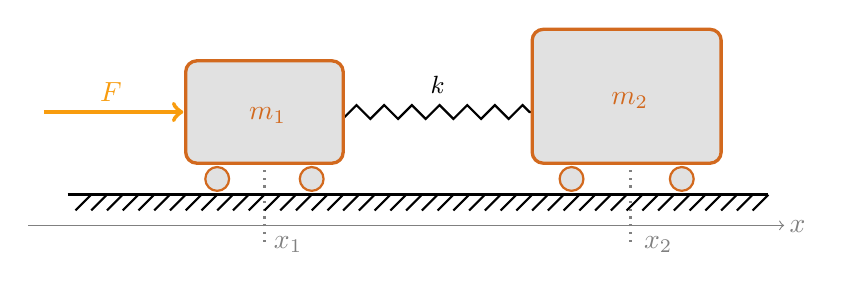
\begin{tikzpicture}%[scale=1.0, xshift= 1cm, yshift= -1.3cm]  
  % Variablen
  \draw[ultra thick, yellow!20!orange, ->] (0.2, 1.05) -- (1.97, 1.05); 
  \node[yellow!20!orange] at (1.05, 1.3) {$F$}; 
%   \draw[very thick, gray] (0.5, -0.4) -- (0.5, -1);
%   \draw[thick, gray] (0.5, -0.6) -- (3.0, -0.6); 
%   \draw[thick, gray] (3.0, -0.55) -- (3.0, -0.65); 
  \draw[thick, dotted, gray] (3.0, -0.6) -- (3.0, 0.4);
  \node[gray] at (3.3, -0.63) {$x_1$}; 
%   \draw[thick, gray] (0.5, -0.8) -- (7.45, -0.8); 
%   \draw[thick, gray] (7.45, -0.75) -- (7.45, -0.85); 
  \draw[thick, dotted, gray] (7.65, -0.6) -- (7.65, 0.4);
  \node[gray] at (8.0, -0.63) {$x_2$}; 
  % Axis
  \draw[gray, ->] (0, -0.39) -- (9.6, -0.39);
%   \draw[gray, ->] (0, -0.4) -- (0, 0.5);
  \node[gray] at (9.77, -0.4) {$x$};
  % Feder  
  \node at (5.2, 1.4) {\small $k$}; 
  \draw[thick, snake] (3.73, 1.05) -- (6.45, 1.05); 
  % Wagen 1
  \draw[myRed1, very thick, fill=myLGray, rounded corners] (2, 0.4) -- (4, 0.4) -- (4, 1.7) -- (2, 1.7) -- cycle;
  \node[myRed1] at (3.04, 1.0) {$m_1$}; 
  % Wagen 2
  \draw[myRed1, very thick, fill=myLGray, rounded corners, xshift=4.4cm] (2, 0.4) -- (4.4, 0.4) -- (4.4, 2.1) -- (2, 2.1) -- cycle;
  % \node[myRed1, xshift=4.4cm] at (3.24, 1.2) {$m_2$}; 
  \node[myRed1] at (7.64, 1.2) {$m_2$}; 
  \foreach \x in {2.4, 3.6, 6.9, 8.3} {
    \path[draw=myRed1, thick, fill=myLGray] (\x, 0.2) circle (1.0ex);
  }
  % Untergrund
  \draw[very thick] (0.5, 0) -- (9.4, 0);
  \foreach \x in {0.8, 1, ..., 9.4} {
    \draw[thick] (\x, 0) -- (\x-0.2, -0.2);
  } 
\end{tikzpicture} 


\caption{Illustration of a $2$-body mass-spring chain moved by an input force $F$.}
\label{fig_2Car_example}
\end{figure}

We consider the DAE in the variables $x_1$, $x_2$, and $F$,
\begin{subequations}
\label{eqn_twocar}
\begin{align}
    m_1\ddot x_1(t) &= \phantom{-} k \big(x_2(t) - x_1(t) - 0.5 \big) + F(t), \label{eqn_twocar_b}\\
  m_2 \ddot x_2(t)&= - k \big(x_2(t) - x_1(t) - 0.5 \big), \label{eqn_twocar_a}\\
        x_2(t) &= \phantom{-} g(t), \label{eqn_twocar_c}
\end{align}
\end{subequations}
which derives from the task to steer a mass $m_2$ along a trajectory $g$ via acting on a connected mass $m_1$ through an unknown force $F$; cf. Figure \ref{fig_2Car_example}. The connection is given by a spring with a constant $k$.

{\bf A Solution and the Index of the State Equations}

Transfer the system \eqref{eqn_twocar} to a first order system $E\dot z = A z + f$ and determine the index of the resulting matrix pair $(E, A)$. What does this mean for the target trajectory $g$? Derive $F$ analytically.
\smallskip

{\bf B Index Reduction by Minimal Extension}

Use the approach of \emph{Minimal Extension} to derive an equivalent representation of \eqref{eqn_twocar} with a lower index.
\smallskip

{\bf C \emph{Radau IIa} Schemes}
The $1$- and the $2$-stages \emph{Radau IIa} schemes are given as 
\smallskip

\begin{minipage}[t]{.3\textwidth}
	\centering
		\begin{tabular}{c|c}
			$1 $ &$1$ \\
			\hline
			&$ 1$\\
		\end{tabular}
\end{minipage} and
\begin{minipage}[t]{.3\textwidth}
	\centering
	\begin{tabular}{c|cc}
		$\frac 13 $ &$ \frac 5{12}$ &$-\frac 1{12}$ \\
		$1$ &$ \frac 34 $ &$ \frac 14$\\
		\hline
		&$ \frac 34 $ &$ \frac 14$\\
	\end{tabular}
\end{minipage}.

Show that for the $2$-stage scheme, the constants defined in Theorem $5.10$ are given as $\kappa_1=\infty$ and $\kappa_2 = 2$.

\vfill

\begin{flushright}
	Please turn the sheet.
\end{flushright}

\newpage
{\bf Coding Exercises}
Implement a numerical time stepping scheme as described in Exercise 4. (You may use and extend the implementation that is for download on the website).
\begin{enumerate}
	\item Use the \emph{Implicit Euler} scheme to integrate the equations modelling the evolution of the pendulum:
		\begin{subequations}\label{eq:pend}
			\begin{align}
				m\ddot x &= - 2(x-r_x)\lambda, \\
				m\ddot y &= - 2(y-r_y)\lambda - mg, \\
				0 &= (x-r_x)^{2} + (y-r_y)^2 - l^2, \label{eq:pendholo}
			\end{align}
		\end{subequations}
		for suitable parameters $m$, $r=(r_x, r_y)$, $l$, and $g$ and suitable initial positions and velocities.

	\item Use the \emph{Implicit Euler} scheme to integrate \eqref{eq:pend} in the (theoretically) equivalent reformulation, where \eqref{eq:pendholo} is replaced by 
		\begin{equation*}
			0 = 2(x-r_x)\dot x + 2(y-r_y)\dot y.
		\end{equation*}
		Evaluate the actual constraint \eqref{eq:pendholo} at the computed values and interprete your observations.
	\item Use the 2-stage \emph{Radau IIa} scheme to integrate the equations modelling the mass-spring chain \eqref{eqn_twocar}, with the following parameters
%
\[
  m_1 = 2 kg,\qquad 
  m_2 = 1 kg, \qquad
  k = 1 \tfrac Nm, \qquad 
  d = 0.5m.
\]
%
initial conditions
\[
  x_1(0) = 0 m,\ \dot x_1(0)  = 0 \tfrac ms, \qquad
x_2(0) = 0.5 m,\ \dot x_2(0) = 0 \tfrac ms.
\]
%
and the target trajectory defined via the start and $g_0 = 0.5m$ terminal positions $g_f = 2.5m$, and the manoeuvre $[0, 4s]$ via 
%
% 126 (t/T)^5 - 420 (t/T)^6 + 540 (t/T)^7 - 315 (t/T)^8 + 70 (t/T)^9
% 1716*s**7 - 9009*s**8 + 20020*s**9 - 24024*s**10 + 16380*s**11 - 6006*s**12 + 924*s**13
\begin{align*}
% \label{eqn_trajectory_rest2rest}
 g(t) = 
 \begin{cases}
	 g_0, 	& \text{if }0\leq t < 1, \\
	 g_0 + p\big(\frac{t-1}{2} \big) (g_f-g_0), 	& \text{if }1\leq t \leq 3, \\
	 g_f, 	& \text{if } 3 < t \leq 4,
 \end{cases}
\end{align*}
with the polynomial

%
\[
  p(s) = 1716 s^7 - 9009s^8 + 20020s^9 - 24024s^{10 }+ 16380s^{11 }- 6006s^{12 }+ 924s^{13}.
\]
%

	\item Use the 2-stage \emph{Radau IIa} and the scheme to integrate the equations modelling the mass-spring chain \eqref{eqn_twocar} having applied the index reduction of \textbf{B}.
	\item Use the 2-stage \emph{Radau IIa} scheme to integrate the equations \eqref{eq:pend} modelling the evolution of the pendulum. 
\end{enumerate}

\end{document}
